\documentclass[tikz,border=12pt]{standalone}
\usepackage[T1]{fontenc}
\usepackage{mathpazo}
\usepackage{amsmath,amssymb}
\usetikzlibrary{arrows.meta, positioning, calc, decorations.pathreplacing}

\definecolor{stblue}{HTML}{7B97AD}
\definecolor{rwgold}{HTML}{B8995E}
\definecolor{sage}{HTML}{7A9A7E}
\definecolor{dkbrown}{HTML}{3D3530}
\definecolor{wmgray}{HTML}{7B7067}
\definecolor{cream}{HTML}{F9F6F0}
\definecolor{border}{HTML}{D4C9B8}
\definecolor{terracotta}{HTML}{C47A6A}

\begin{document}
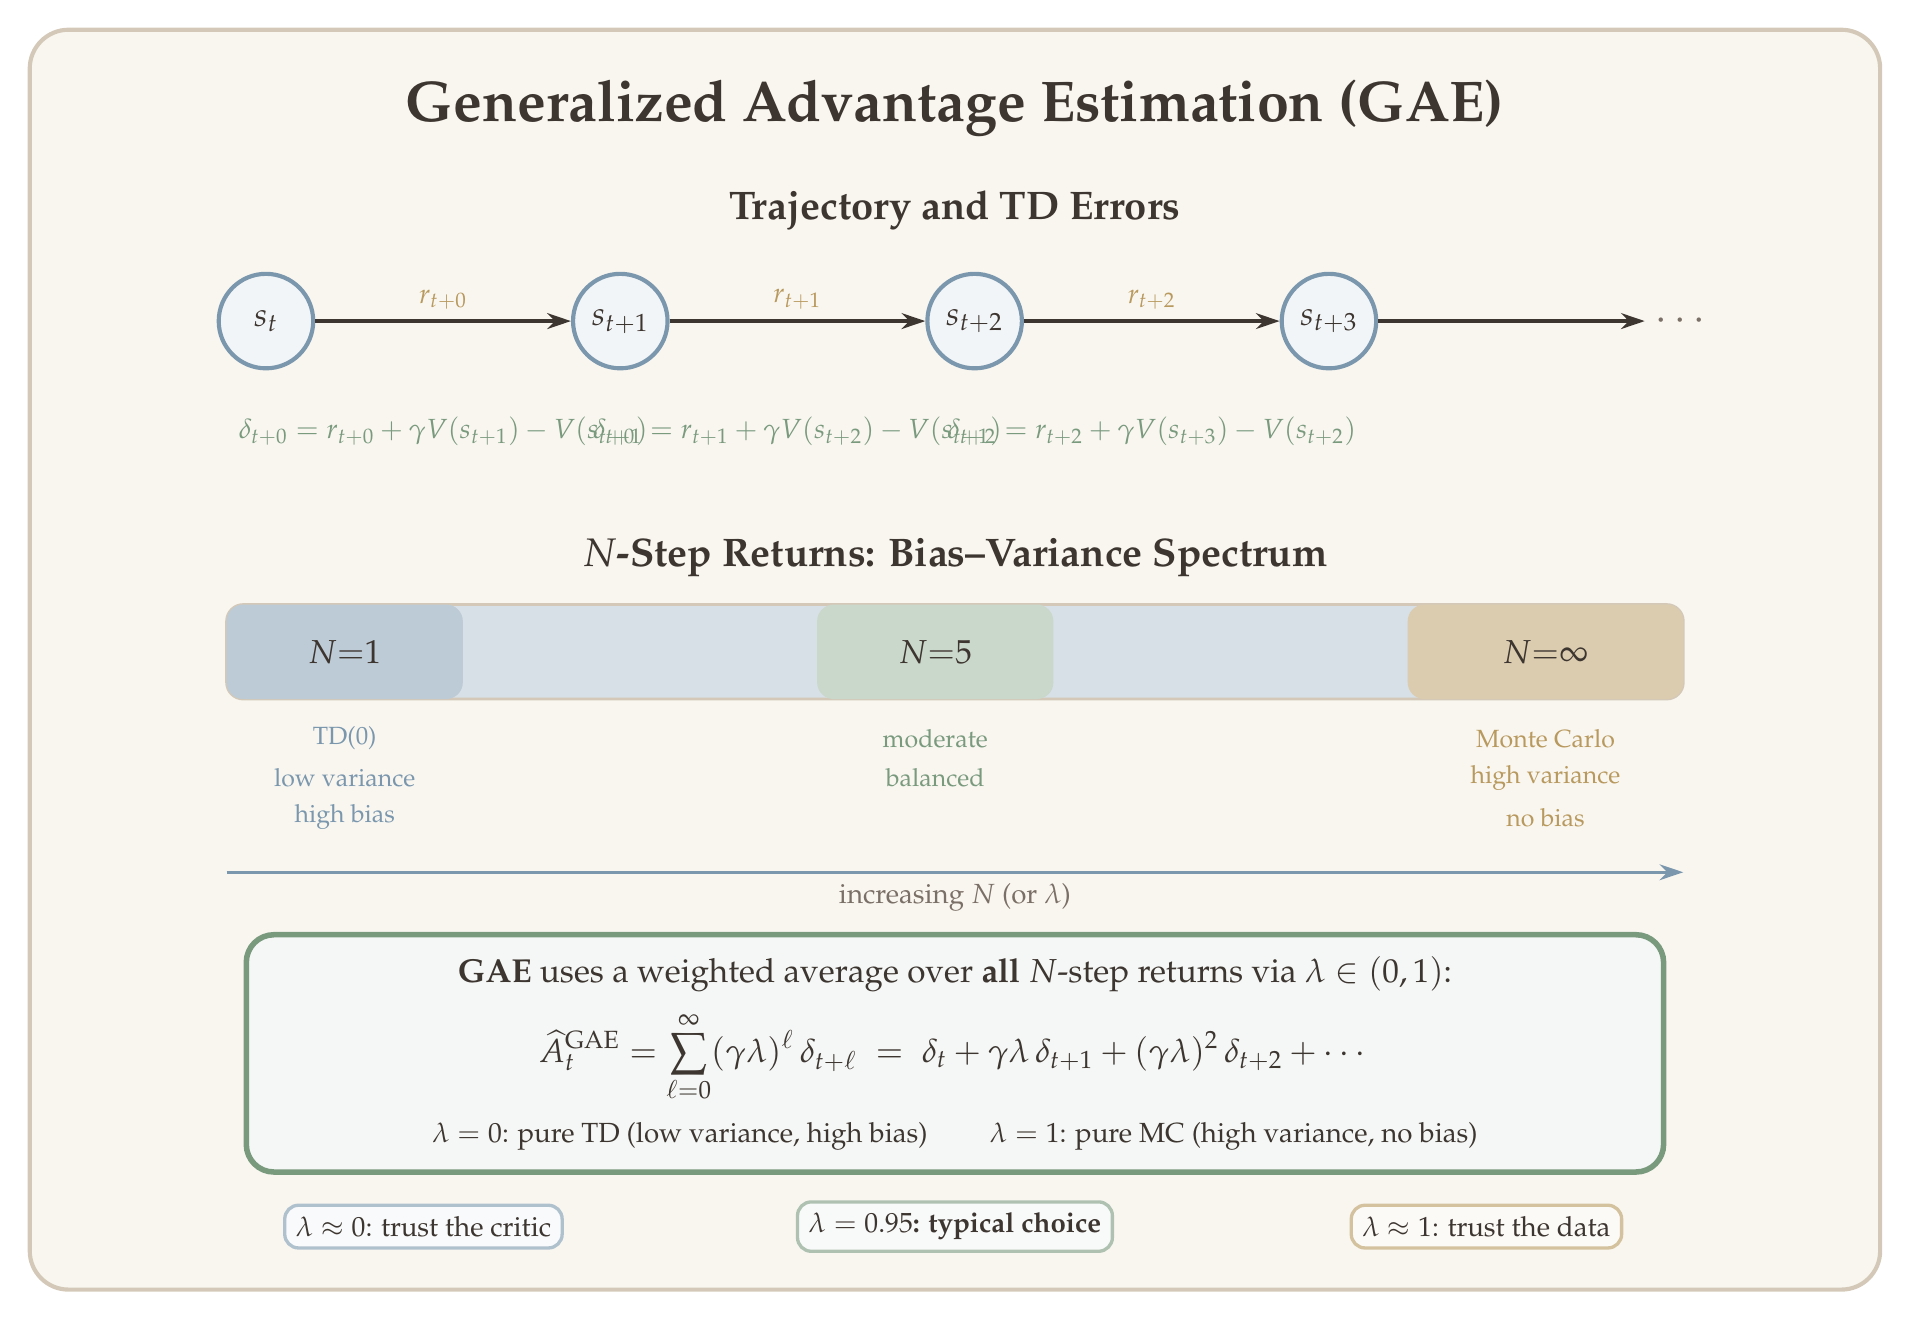
\begin{tikzpicture}[
  >={Stealth[length=3mm, width=2mm]},
]

% Background
\fill[cream, rounded corners=14pt] (-1.5,-5.5) rectangle (22,10.5);
\draw[border, rounded corners=14pt, line width=1.5pt] (-1.5,-5.5) rectangle (22,10.5);

% Title
\node[font=\huge\bfseries, text=dkbrown] at (10.25,9.5)
  {Generalized Advantage Estimation (GAE)};

% =============================================
% Timeline: trajectory with TD errors
% =============================================
\node[font=\Large\bfseries, text=dkbrown] at (10.25,8.2) {Trajectory and TD Errors};

\foreach \i/\lab in {0/$s_t$, 1/$s_{t+1}$, 2/$s_{t+2}$, 3/$s_{t+3}$, 4/$\cdots$} {
  \pgfmathsetmacro{\x}{1.5 + \i * 4.5}
  \ifnum\i<4
    \node[draw=stblue, line width=1.5pt, fill=stblue!10, circle,
          minimum size=12mm, font=\large, text=dkbrown] (s\i) at (\x, 6.8) {\lab};
  \else
    \node[font=\Large, text=wmgray] (s\i) at (\x, 6.8) {\lab};
  \fi
}

% Arrows between states with rewards
\foreach \i [evaluate=\i as \j using int(\i+1)] in {0,1,2} {
  \draw[->, line width=1.5pt, dkbrown] (s\i) -- (s\j)
    node[midway, above, font=\normalsize, text=rwgold] {$r_{t+\i}$};
}
\draw[->, line width=1.5pt, dkbrown] (s3) -- (s4);

% TD errors below arrows
\foreach \i [evaluate=\i as \j using int(\i+1)] in {0,1,2} {
  \pgfmathsetmacro{\x}{1.5 + \i * 4.5 + 2.25}
  \node[font=\normalsize, text=sage, align=center] at (\x, 5.4)
    {$\delta_{t+\i} = r_{t+\i} + \gamma V(s_{t+\j}) - V(s_{t+\i})$};
}

% =============================================
% N-step returns spectrum
% =============================================
\node[font=\Large\bfseries, text=dkbrown] at (10.25,3.8) {$N$-Step Returns: Bias--Variance Spectrum};

% Spectrum bar
\fill[stblue!30, rounded corners=6pt] (1,2.0) rectangle (19.5,3.2);
\draw[border, rounded corners=6pt, line width=1pt] (1,2.0) rectangle (19.5,3.2);

% Gradient fill effect
\fill[stblue!50, rounded corners=6pt] (1,2.0) rectangle (4,3.2);
\fill[sage!40, rounded corners=6pt] (8.5,2.0) rectangle (11.5,3.2);
\fill[rwgold!50, rounded corners=6pt] (16,2.0) rectangle (19.5,3.2);

% Labels on spectrum
\node[font=\large\bfseries, text=dkbrown] at (2.5,2.6) {$N{=}1$};
\node[font=\small, text=stblue] at (2.5,1.5) {TD(0)};
\node[font=\small, text=stblue] at (2.5,1.0) {low variance};
\node[font=\small, text=stblue] at (2.5,0.5) {high bias};

\node[font=\large\bfseries, text=dkbrown] at (10,2.6) {$N{=}5$};
\node[font=\small, text=sage] at (10,1.5) {moderate};
\node[font=\small, text=sage] at (10,1.0) {balanced};

\node[font=\large\bfseries, text=dkbrown] at (17.75,2.6) {$N{=}\infty$};
\node[font=\small, text=rwgold] at (17.75,1.5) {Monte Carlo};
\node[font=\small, text=rwgold] at (17.75,1.0) {high variance};
\node[font=\small, text=rwgold] at (17.75,0.5) {no bias};

% Arrows
\draw[->, line width=1.2pt, stblue] (1,-0.2) -- (19.5,-0.2)
  node[midway, below, font=\normalsize, text=wmgray] {increasing $N$ (or $\lambda$)};

% =============================================
% GAE formula box
% =============================================
\node[draw=sage, line width=2pt, fill=sage!8, rounded corners=10pt,
      minimum width=180mm, minimum height=26mm,
      font=\large, text=dkbrown, align=center, inner sep=8pt]
  at (10.25,-2.5)
  {\textbf{GAE} uses a weighted average over \textbf{all} $N$-step returns via $\lambda \in (0,1)$:\\[6pt]
   $\displaystyle \widehat{A}_t^{\text{GAE}} = \sum_{\ell=0}^{\infty} (\gamma\lambda)^\ell \, \delta_{t+\ell}
   \;=\; \delta_t + \gamma\lambda\,\delta_{t+1} + (\gamma\lambda)^2\,\delta_{t+2} + \cdots$\\[6pt]
   {\normalsize $\lambda = 0$: pure TD (low variance, high bias) \qquad
   $\lambda = 1$: pure MC (high variance, no bias)}};

% Lambda labels
\node[draw=stblue!60, line width=1.2pt, fill=stblue!5, rounded corners=5pt,
      font=\normalsize, text=dkbrown, inner sep=4pt]
  at (3.5,-4.7) {$\lambda \approx 0$: trust the critic};
\node[draw=rwgold!60, line width=1.2pt, fill=rwgold!5, rounded corners=5pt,
      font=\normalsize, text=dkbrown, inner sep=4pt]
  at (17,-4.7) {$\lambda \approx 1$: trust the data};
\node[draw=sage!60, line width=1.2pt, fill=sage!5, rounded corners=5pt,
      font=\normalsize\bfseries, text=dkbrown, inner sep=4pt]
  at (10.25,-4.7) {$\lambda = 0.95$: typical choice};

\end{tikzpicture}
\end{document}
